% This is samplepaper.tex, a sample chapter demonstrating the
% LLNCS macro package for Springer Computer Science proceedings;
% Version 2.20 of 2017/10/04
%
\documentclass[runningheads]{llncs}
%
\usepackage{graphicx}
% Used for displaying a sample figure. If possible, figure files should
% be included in EPS format.
%
% If you use the hyperref package, please uncomment the following line
% to display URLs in blue roman font according to Springer's eBook style:
% \renewcommand\UrlFont{\color{blue}\rmfamily}

\begin{document}
%
\title{Direction-Free In-Air Signature Verification Using WIFI CSI Signal}
%
%\titlerunning{Abbreviated paper title}
% If the paper title is too long for the running head, you can set
% an abbreviated paper title here
%
\author{YoungWoong KWON\inst{1} \and
Jooyoung Kim\inst{1} \and
Kar-Ann Toh\inst{1}}
%
\authorrunning{Y. Kwon et al.}
% First names are abbreviated in the running head.
% If there are more than two authors, 'et al.' is used.
%
\institute{Yonsei University \and
\email{lncs@springer.com}\\
\url{http://www.springer.com/gp/computer-science/lncs} \and
ABC Institute, Rupert-Karls-University Heidelberg, Heidelberg, Germany\\
\email{\{abc,lncs\}@uni-heidelberg.de}}
%
\maketitle              % typeset the header of the contribution
%
\begin{abstract}
The abstract should briefly summarize the contents of the paper in
15--250 words.

\keywords{First keyword  \and Second keyword \and Another keyword.}
\end{abstract}
%
%
%
\section{Introduction}

\subsection{Motivation}
i. Pros of In-Air WIFI CSI signature system
1) Cheap: Use commercial device
2) Easy: No additional devices is needed
3) Secure: Hard to forgery
ii. Cons of In-Air WIFI CSI signature system
1) Setting direction problem
a) Different direction -> Different feature is needed
b) Hard to set exactly same direction as authentication before
Size of signature can varies

\subsection{Contribution}
- Overcome cons of WIFI signature system
- Robust to signal direction, size

\section{Related Works}

\subsection{ConvNets}
% description of convnet
Convolutional Neural Networks is a specal case of Multi Layer Perceptron and it has unified feature extractor and classifier in one network. It has been widely applied to visual objects such as image, video or 2D array input. Several factors make ConvNets attractive in image related tasks.
Local connectivity captures local correlation property of image. It is applycable by using ConvNet filter.Weight sharing helps to reduce the number of weights in feature maps.
Also, CUDA libraries makes the tranining feature maps easier to reduce training time.
%

\subsection{Siamese Networks}

% description of siamese net
In \cite{bromley1994signature}, LeCun et al. Introduced Siamese nets as parts of their handwritten signature verification system. 
A siamese neural network consists of twin networks which accept distinct inputs but are joined by an energy function at the top.\cite{koch2015siamese}
% differences in feature extractor
They proposed a feature extractor based on Time Delay Neural Networks\cite{lang1990time} and feature matcher based on cosine distance of feature vector. 

\section{Proposed System}

%system overview

In this section, we propose a direction-free identify verification system based on the Wi-Fi based in-air handwritten signature which utilizes the Siamese network learning.

An overview of the proposed system is shown in Fig.1.
% Figure 1
\begin{figure}
    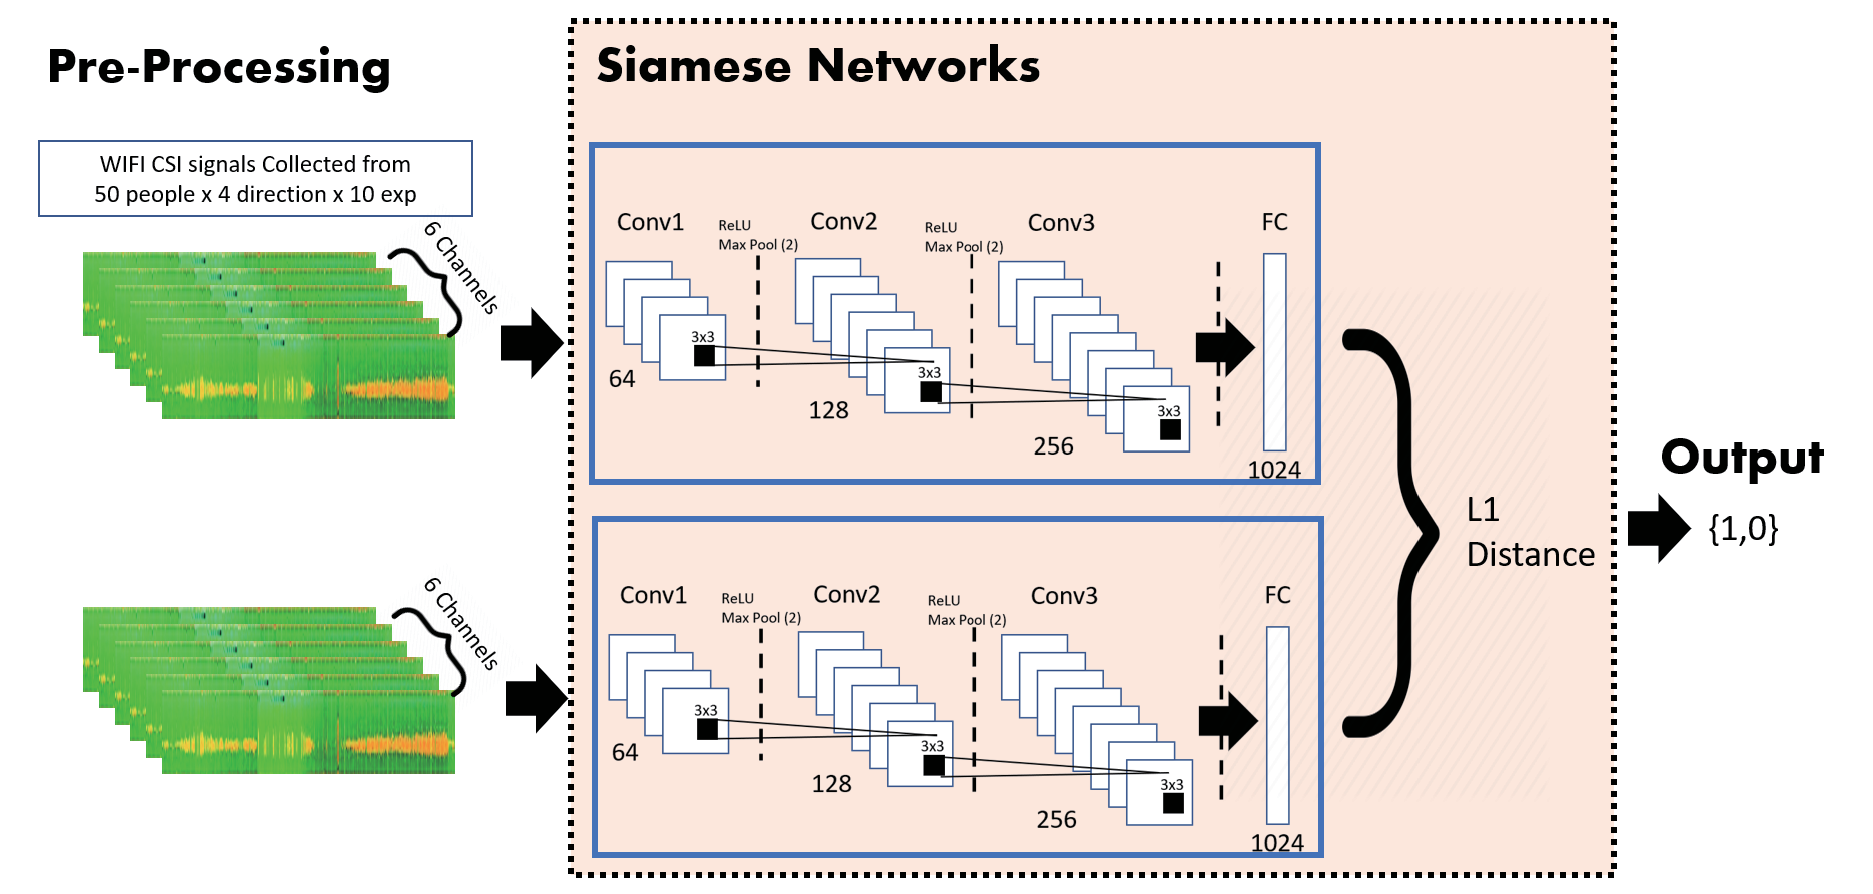
\includegraphics[width=\textwidth]{network2.eps}
    \caption{Structure of Siamese network} \label{network2}
\end{figure}

Essentially, we train the verification model to identify the input pairs according to the probability on whether they belong to the same class or different classes.\cite{koch2015siamese} Subsequently, the 

\iffalse
% main purpose2: direction free
Since signals may differ in the direction in which they are entered, our system must be capable of extracting non-direction-related characteristics from two signals.
\fi

Even if a signal belongs to the same class, the shape of the input is very different if the signal is oriented differently.
To classify regardless of the direction of the signal, we focused on the model shall be capable of extracting features unrelated to the direction.

%% Pre-processing
\subsection{Data Preprocessing}

In order to be used as an input to a siamese network, the signal must be pre-processed.

% used only abs value
First, the signal has to be converted to non-complex form.
Since the Wi-Fi signature signals in CSI packets in 2.4Ghz has firmware issues in their phase \cite{wang2015understanding}. we used only absolute value.

% preprocessing
% From HC's Papaer
Second, all inputs must be arranged of the same size.
Since all signals have different length, the gradient operation with respect to the time instance is adapted to measure the short time energy. 
Data points with the highest short-time energy within the time period are regarded as the starting and the ending points of the in-air signature.
And they are re-sampled uniformly based on Fast Fourier Transform (FFT)  to normalize the length of the data. \cite{moon2017air}% HC's end

% Methods 
% Section: Feature Extraction
\subsubsection{Convolutional Neural Network for Feature Extraction}

% structure of siamese network
To perform the feature extraction, we first need to have convolutional neural networks to serve as the feature extractor
Based on the ConvNet structure.\cite{lecun1998gradient} 

% structure of siamese network
When two processed signals come as the input, they are put to 2 symmetric ConvNet. 
%Symmetric Architecture
Some of the features CNN extracted are related to the shape of the signature, but CNN's features are not just those that help to classify signatures. some may be heavily influenced by the direction in which the signature was entered. Structure of the network is shown in Fig.2.
% Figure 2

% weight tying
We aim to classify the signature in a direction that is not related to the direction in which it was entered. This type of property interferes with the classification of signatures.
To focus on characteristics conducive to classification, The two CNN networks are arranged side by side symmetrically.
It was also designed to have the same weight on the symmetrical CNN network.


% sister networks
This feature extractor is composed of two sister network, which are identical ConvNets with the exact same weights

% CNN: purpose
Purpose of ConvNet in our model is to extract a feature vector from the CSI signal. 

% parameters of convnet
this ConvNets are consists of a number of consecutive convolution layers with active functions, and a pooling layer in the end.
the Convolution Layer has n convolution filters in it.

% functions of convnet
Their weights are tied to extract the same characteristics from signals in different directions.
By sharing their feature map, this ConvNet is trained to learn characteristics regardless of the direction.

% outputs feature vector
Through a convolution filter, each CSI signal is transformed into a feature vector. this entire process is jointly optimized by backpropagation.



\subsection{Siamese Network For.}

% Functions of Siamese in our system
% Introduce Siamese Net

Siamese neural networks employ a unique structure to naturally rank similarity between inputs. It can discriminate between the class-identity of image pairs.
\cite{koch2015siamese}

Two preprocessed signals enter the Siamese network and the network extracts non-directional characteristics from two signals and calculates how similar the two extracted characteristics are. The model outputs the probability that the two signals are of the same class. %it is learned by the back-propagation.
This network consists of feature extraction and feature matching part.

\subsubsection{Feature Matching}

% Use L1 distances of Feature vector of 2 input images
% From HC's In-Air paper below:
Let $\mathbf{m}\in{\mathrm{R}}^{d\times1}$ and $\mathbf{n}\in{\mathrm{R}}^{d\times1}$ be feature vectors extracted from two samples.
The L-1 distance between the two features can be calculated as  follows:
Where $\mathbf{p}$ denotes the L-1 distance. In the Siamese networks, this L-1 distance is utilized to match between two feature vectors.

% From HC's End
% From Oneshot paper below
\begin{equation}
    \mathbf{p} = 
    \sigma(\sum_j\alpha_{j}\mid
    \mathbf{m}_{1,L-1}^{(j)} - 
    \mathbf{n}_{1,L-1}^{(j)}\mid)  
\end{equation}
where σ is the sigmoidal
activation function. This final layer induces a metric on the learned feature space of the (L − 1)th hidden layer and scores the similarity between the two feature vectors. The αj are additional parameters that are learned by the model during training, weighting the importance of the component-wise distance. This defines a final Lth fully-connected layer for the network which joins the two Siamese twins.
% From oneshot end

The output of the CNN is feature vectors extracted from two samples. The Euclidean distance between the two features can be calculated.
In the proposed system, this Euclidean distance is utilized to match between two feature vectors.


\section{Experiments}

\subsubsection{Loss and Backpropagation}
 We impose a regularized cross-entropy objective on our binary classifier.
This objective is combined with standard backpropagation algorithm, where the gradient is additive across the twin networks due to the tied weights.
 We initialized all network weights in the convolutional layers from a normal distribution with zero-mean and a standard deviation of 10−2. Biases were also initialized from a normal distribution, but with mean 0.5 and standard deviation 10−2.

\section{Conclusion}

%
% ---- Bibliography ----
%
% BibTeX users should specify bibliography style 'splncs04'.
% References will then be sorted and formatted in the correct style.
%
%\bibliographystyle{splncs04}
%\bibliography{mybibliography}
%


%\begin{thebibliography}{8}

\bibliographystyle{splncs04}
\bibliography{bib_acpr}

%\end{thebibliography}

\end{document}




%% Template End
\section{*** Template ***}
\section{First Section}
\subsection{A Subsection Sample}
Please note that the first paragraph of a section or subsection is
not indented. The first paragraph that follows a table, figure,
equation etc. does not need an indent, either.

Subsequent paragraphs, however, are indented.

\subsubsection{Sample Heading (Third Level)} Only two levels of
headings should be numbered. Lower level headings remain unnumbered;
they are formatted as run-in headings.

\paragraph{Sample Heading (Fourth Level)}
The contribution should contain no more than four levels of
headings. Table~\ref{tab1} gives a summary of all heading levels.

\begin{table}
\caption{Table captions should be placed above the
tables.}\label{tab1}
\begin{tabular}{|l|l|l|}
\hline
Heading level &  Example & Font size and style\\
\hline
Title (centered) &  {\Large\bfseries Lecture Notes} & 14 point, bold\\
1st-level heading &  {\large\bfseries 1 Introduction} & 12 point, bold\\
2nd-level heading & {\bfseries 2.1 Printing Area} & 10 point, bold\\
3rd-level heading & {\bfseries Run-in Heading in Bold.} Text follows & 10 point, bold\\
4th-level heading & {\itshape Lowest Level Heading.} Text follows & 10 point, italic\\
\hline
\end{tabular}
\end{table}


\noindent Displayed equations are centered and set on a separate
line.
\begin{equation}
x + y = z
\end{equation}
Please try to avoid rasterized images for line-art diagrams and
schemas. Whenever possible, use vector graphics instead (see
Fig.~\ref{fig1}).

\begin{figure}
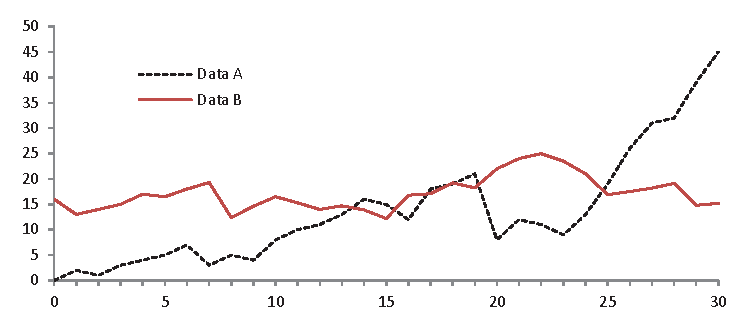
\includegraphics[width=\textwidth]{fig1.eps}
\caption{A figure caption is always placed below the illustration.
Please note that short captions are centered, while long ones are
justified by the macro package automatically.} \label{fig1}
\end{figure}

\begin{theorem}
This is a sample theorem. The run-in heading is set in bold, while
the following text appears in italics. Definitions, lemmas,
propositions, and corollaries are styled the same way.
\end{theorem}
%
% the environments 'definition', 'lemma', 'proposition', 'corollary',
% 'remark', and 'example' are defined in the LLNCS documentclass as well.
%
\begin{proof}
Proofs, examples, and remarks have the initial word in italics,
while the following text appears in normal font.
\end{proof}
For citations of references, we prefer the use of square brackets
and consecutive numbers. Citations using labels or the author/year
convention are also acceptable. The following bibliography provides
a sample reference list with entries for journal
articles~\cite{ref_article1}, an LNCS chapter~\cite{ref_lncs1}, a
book~\cite{ref_book1}, proceedings without editors~\cite{ref_proc1},
and a homepage~\cite{ref_url1}. Multiple citations are grouped
\cite{ref_article1,ref_lncs1,ref_book1},
\cite{ref_article1,ref_book1,ref_proc1,ref_url1}.
%
% ---- Bibliography ----
%
% BibTeX users should specify bibliography style 'splncs04'.
% References will then be sorted and formatted in the correct style.
%
% \bibliographystyle{splncs04}
% \bibliography{mybibliography}
%
\begin{thebibliography}{8}
\bibitem{ref_article1}
Author, F.: Article title. Journal \textbf{2}(5), 99--110 (2016)

\bibitem{ref_lncs1}
Author, F., Author, S.: Title of a proceedings paper. In: Editor,
F., Editor, S. (eds.) CONFERENCE 2016, LNCS, vol. 9999, pp. 1--13.
Springer, Heidelberg (2016). \doi{10.10007/1234567890}

\bibitem{ref_book1}
Author, F., Author, S., Author, T.: Book title. 2nd edn. Publisher,
Location (1999)

\bibitem{ref_proc1}
Author, A.-B.: Contribution title. In: 9th International Proceedings
on Proceedings, pp. 1--2. Publisher, Location (2010)

\bibitem{ref_url1}
LNCS Homepage, \url{http://www.springer.com/lncs}. Last accessed 4
Oct 2017
\end{thebibliography}
\end{document}




% old parts

% Meaning of CSI
%[From Halperin paper]
CSI captures signal strength and phase information for OFDM subcarriers and between each pair of transmit-receive antennas.
It runs on a commodity 802.11n NIC, and records Channel State Information (CSI) based on the 802.11 standard.
The CSI contains information about the channel between sender and receiver at the level of individual data subcarriers, for each pair of transmit and receive antennas.
%[From Halperin End]

% Structure of CSI
%[From HC's ELM paper]
In a frequency domain, the CSI of sub-carrier $\mathbf{c}$ between transmitter(Tx) and receiver(Rx) can be modeled as 
$\mathnormal{R}_{c} = \mathbf{H}_{c}\mathnormal{T}_{c} +\mathnormal{N}$ where the $\mathnormal{R}_{c}$ and $\mathnormal{T}_{c}$  denote the received and the transmitted signal vector of dimension $\mathnormal{r}$ and $\mathnormal{t}$, respectively. The $\mathnormal{N}$ is the additive channel noise and $\mathbf{H}_{c}$ is the $\mathnormal{r}\times\mathnormal{t}$ channel matrix. The CSI of sub-carrier $\mathnormal{c}$ can be modeled as follows:
\begin{equation}
    \mathnormal{h}_{c} = \mid\mathnormal{h}_{c}\mid\mathnormal{e}^{\angle\theta},
\end{equation}
where $\mid\mathnormal{h}_{c}\mid$ and $\theta$ represent the amplitude and the phase of the sub-carrier, respectively.
%[From HC's ELM end]


% description of siamese
In this paper, we propose a for signature verification system that is applicable for WIFI CSI signal, which is more complex and larger than handwritten images. 
% advantages of using Convnet filter
Based on Convnets as feature extractor, we are able to make feature vector from CSI signal reflecting local connectivity between signals at a near frequency range and closer measurement time. 
The proposed method achieved better performance because it is applicable to all points of CSI signals. This is due to the weight sharing the property of the Convnet filter.
